\documentclass{article}

\usepackage[utf8]{inputenc}
\usepackage[0T1]{fontenc}
\usepackage[french]{babel}
\usepackage{natbib}
\usepackage{graphicx}
\usepackage{setspace}
\usepackage{amssymb}
\usepackage[a4paper,bindingoffset=0.2in,%
            left=1in,right=1in,top=1in,bottom=1in,%
            footskip=.25in]{geometry}
\onehalfspacing

\begin{document}
    \begin{center}
        \rule{1.05\textwidth}{2pt}\\
            \Huge Mémoire de projet de data mining\\
            \huge \textbf{Sujet : Analyse des relevés des notes des étudiants de l'ENSIAS}\\
        \rule{1.05\textwidth}{2pt}\\
    \thispagestyle{empty}
    \end{center}
\newpage
\thispagestyle{plain} % empty
\thispagestyle{empty}
\mbox{}
    \newpage
    \begin{center}
    \Large \textbf{Remerciement}
    \end{center}
    \begin{spacing}{2}
    \par Nous profitons par le biais de ce rapport pour exprimer nos vifs remerciements à toute personne contribuant de près ou de loin à l’élaboration de ce travail.
    \par Nous tenons à remercier vivement tous nos professeurs. Le Directeur de notre établissement Mr Mohammed HALIM, qui ont contribué à la réalisation de ce modeste projet, qui nous ont encadrés et aidés tout au long de notre parcours. Ainsi nous remercions l’administration de l’École Nationale Supérieure d’Informatique et d’Analyse des Systèmes qui à travers leur programme nous ont fourni des outils de qualité facilitant notre spécialisation. 
    \par Un merci bien particulier adressé également à Mme. Houda BENBRAHIM notre professeur  de Data mining, pour ces remarques, ses directives, et l’intérêt qu’elle porte à ses étudiants. Nous tenons à lui exprimer nos sincères remerciements pour son suivi et ses orientations.
    \end{spacing}
    \newpage 
    \tableofcontents
    \newpage 
    \listoffigures
    \listoftables
    \newpage
    \begin{center}
    \Large \textbf{Introduction}
    \end{center}
    \begin{spacing}{2}
    \par Dans notre école l’ENSIAS, on travaille plusieurs projets dans des groupes de deux à six personnes de façon collaborative et responsable. Le travail de groupe développe bien sûr les compétences sociales, mais il poursuit aussi l’objectif d’intensifier l’apprentissage disciplinaire. Pour cela, nous devons bien choisir notre groupe. Les enseignants laissent aux élèves la liberté de former leurs groupes. En général, les groupes sont formés en basant sur l’amitié qui relie les élèves et non pas leurs compétences.
    \par Le but de ce projet est d’aider les élèves à former des groupes en exploitant intelligemment leurs relevés des notes de la première et la deuxième année et extraire des groupes de personnes ayant plus ou moins les mêmes notes dans les différentes matières. Donc nous obtenons des groupes homogènes de personnes qui peuvent exploiter leurs points fort communs pour réaliser un bon projet.
    \par Dans ce projet on va suivre la méthode CRISP-DM qui signifie « Cross-industry standard process for data mining ». Chaque chapitre va être une étape de cette méthode. Donc nous aurons cinq chapitres dans ce rapport qui sont : la compréhension métier, la compréhension des données, la préparation des données, la  modélisation et enfin l’évaluation et le déploiement.
    \end{spacing}
    \newpage
        \section{La compréhension métier}
            Cette première phase consiste à bien comprendre les éléments métiers et la problématique qu’on vise à résoudre. On va commencer par déterminer les objectifs stratégiques et opérationneles. Puis, on va évaluer la situation actuelle. Finallement, vient la traduction de l’objectif stratégique en concepts de Data mining.\\
            \subsection{Détermination des objectifs stratégiques et opérationnelles}
                Le problème qu’on rencontre dans le travail de groupe dans notre école l’ENSIAS c’est la non homogénéité des groupes. Le seul facteur de la formation de ces groupes c’est la relation entre les membres. Ainsi les outils techniques peuvent ne pas plaire tous les membres d’un groupe. D’où vient l’idée de notre projet, former des groupes homogènes des étudiants ayant les mêmes compétences pour qu’ils puissent travailler sur un projet qui exploite leurs compétences communes. Tous cela, en analysant leurs résultats et chercher les élèves ayant des résultats similaires dans la même filière.\\
            \subsection{Analyse de la situation actuelle}
                Actuellement, nous disposons de quelques relevés de notes de la deuxième année de quelques filières : la filière e-Management et Business Intelligence (eMBI), la filière Génie Logiciel (GL) et les notes de la première année. Tous ces relevés de notes sont de la promotion de l’année 2020. Nous devons encore collecter les relevés de notes d’autres filières : la filière Ingénierie e-Logistique (IeL), la filière Ingénierie des Systèmes Embarqués et Mobiles (ISEM) et la filière Sécurité des Systèmes d'Information (SSI).\par
                Parmi les problèmes que nous avons rencontrés c’est la sensibilité des données. On ne peut pas diffuser telles données personnelles, donc on doit cacher les noms et les prénoms des étudiants pour protéger leurs confidentialités.\\
            \subsection{Détermination des objectifs du Data Mining}
                Puisque l’objectif stratégique est clairement défini, il convient maintenant de le traduire en concepts de Data Mining. On va opter à une technique descriptive car nous sommes en train de présenter une information cachée par le volume des données. Et plus spécifiquement on va travailler un problème de clustering qui sert à regrouper des données non étiquetées présentant des propriétés similaires. Dans notre cas les propriétés sont les notes de chaque module.\\
                \subsubsection{Clustering}
                    Le Clustering ou le partitionnement des données est une méthode de classification non supervisée rassemble un ensemble d’algorithmes d’apprentissage pour relever des sous-ensembles des données difficiles à identifier à l’œil nu.\par
                    Pour atteindre ce but, cette technique vise à maximiser l’inertie entre les sous-ensembles pour bien les différencier et minimiser celle au sein du même ensemble pour qu’il soit plus homogène. Il existe plusieurs méthodes de clustering : méthodes hiérarchiques, méthodes de partitionnement et méthode mixtes.\\
                \subsubsection{K-means}
                    Nous avons  choisis travailler avec l’algorithme de K-means c’est un algorithme de partitionnement qui permet de regrouper les observations de notre data set en K clusters distincts. L’algorithme de K-means est comme suit :\\
                    \begin{figure}[h!]
                        \centering
                        \fbox{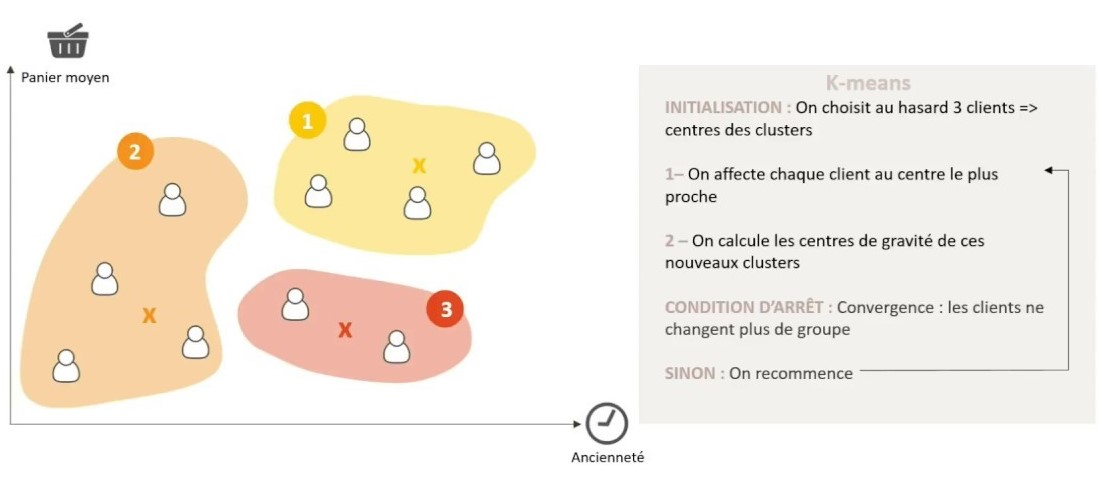
\includegraphics[scale=0.5]{kmeans}}
                        \caption{Principe algorithmique de K-means}
                        \label{fig:1}
                    \end{figure}
    \newpage
        \section{La compréhension des données}
            La phase de compréhension des données de CRISP-DM implique l’étude des données disponibles pour le Data mining. On doit tout d’abord collecter les données puis faire la description de ces données. La troisième étape est l’exploration des données et comme étape finale vérifier la qualité des données collectées.\\
            \subsection{Collecte des données}
                Nous avons pu collecter les notes de toute la promotion 2020 dans toutes les filière sauf la filière (IWIM) auprès des élèves de cette promotion. Les notes de la première année qui est une année commune à toutes les filières. Puis les notes des élèves de chaque filière : eMBI, GL, IeL, SSI, et ISEM en deuxième année.\par
                \begin{figure}[h!]
                    \centering
                    \fbox{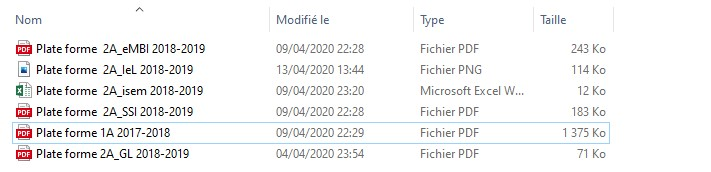
\includegraphics[scale=0.8]{data}}
                    \caption{Les données collectées}
                    \label{fig:2}
                \end{figure} 
                Nos fichiers sont de différents formats : des fichiers pdf, un fichier png et un fichier Microsoft Excel.\\
            \subsection{Description des données}
                Chaque fichier contient le nom et le prénom de l’étudiant, le moyen dans chaque semestre et chaque module ainsi la décision finale.\\
                \begin{figure}[h!]
                    \centering
                    \fbox{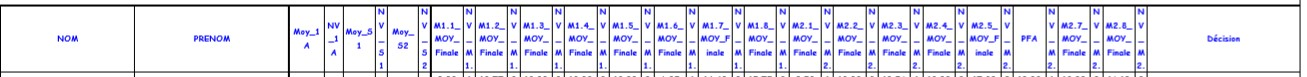
\includegraphics[scale=0.45]{columns}}
                    \caption{Les composants de chaque fichier}
                    \label{fig:columns}
                \end{figure} 
                \begin{table}
                    \begin{tabular}{|p{3cm}|p{6cm}|p{2cm}|p{2cm}|}
                        \hline
                        Code & Signification & Type & Longueur \\ \hline
                        NOM & Le nom de l’étudiant. & Texte & 32 \\  \hline
                        PRENOM & Le prénom de l’étudiant. & Texte & 32 \\ \hline
                        Moy\_1A & Le moyen de la première année. & Numérique & 5 \\  \hline
                        Moy\_S1 & Le moyen de la première semestre de la première année. & Numérique & 5 \\  \hline
                        Moy\_S2 & Le moyen de la deuxième semestre de la première année. & Numérique & 5 \\  \hline
                        NV\_1A & Le nombre des modules non validé dans la première année .& Numérique & 2 \\  \hline
                        NV\_S1 & Le nombre des modules non validé dans la première semestre de la première année. & Numérique & 1 \\ \hline
                        NV\_S2 & Le nombre des modules non validé dans la deuxième semestre de la première année. & Numérique & 1 \\ \hline
                        Mx.y\_MOY\_Finale & Le moyen du yème module dans la xème semestre. & Numérique & 5 \\  \hline
                        NV_Mx.y & Le module y de la xème semestre est-il valide ?
                        \begin{itemize}
                            \item 0 : si le module est validé (Mx.y-MOY-Finale >= 12).
                            \item 1 : si le module n’est pas validé.
                        \end{itemize} & Numérique & 5 \\  \hline
                        PFA & La note du projet de la fin de l’année. & Numérique & 5 \\  \hline
                        Décision & La décision du conseil il prend 6 valeurs :
                        \begin{itemize}
                            \item Félicitation si  $Moy\_1A\ge15$.
                            \item Encouragement si $15<Moy\_1A\le14$.
                            \item Admis si $14<Moy\_1A\le12$ et $NV1A\le4$.
                            \item Admis avec indulgence si $12<Moy\_1A\le min\_moy$ ou $NV\_1A>4$.
                            \item Ajourné si $min\_moy<Moy\_1A$ (min\_moy est décidé par le conseil).
                            \item Réorienté si l’étudiant n’était pas admis pendant deux ans.
                        \end{itemize} & Texte & 32 \\ 
                        \hline
                    \end{tabular}
                    \caption{Dictionnaire des données}
                    \label{table:1}
                \end{table}
        \newpage
        \subsection{Exploration des données}
            Pour explorer les données il faut tout d’abord transformer nos fichiers en un format adopter par le Spss modeler. Nous avons trois formats : des fichiers excel adopter par le Spss modeler et des fichiers PDF et une image. Pour les fichiers PDF nous avons pu les convertir en fichiers excel facilement. Par contre la conversion de l’image a été faite manuellement puisque sa qualité était mauvaise.\par
            \begin{figure}[h!]
                \centering
                \fbox{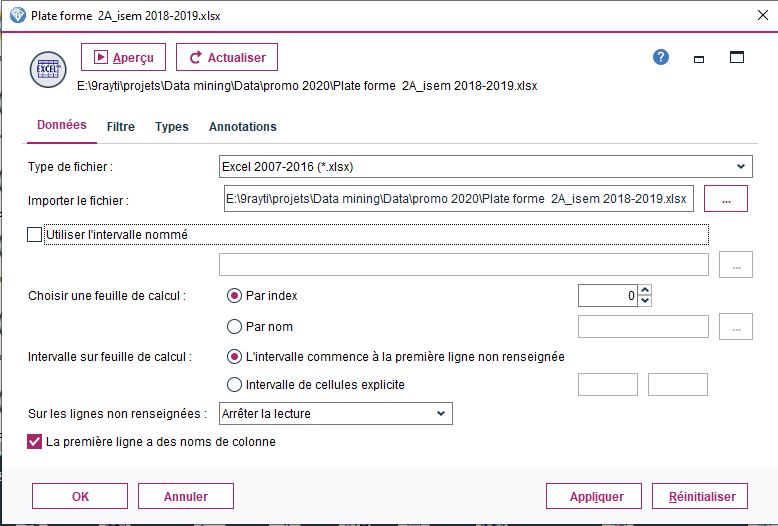
\includegraphics[scale=0.6]{fig4}}
                \caption{Création des nœuds sources}
                \label{fig:4}
            \end{figure}
            Nous avons placé des nœuds sources excel et nous avons édité les nœuds en important les fichiers excel qui contiennent les données. 
            \subsubsection{Exploradion à l’aide des tableaux}
                \begin{figure}[h!]
                    \centering
                    \fbox{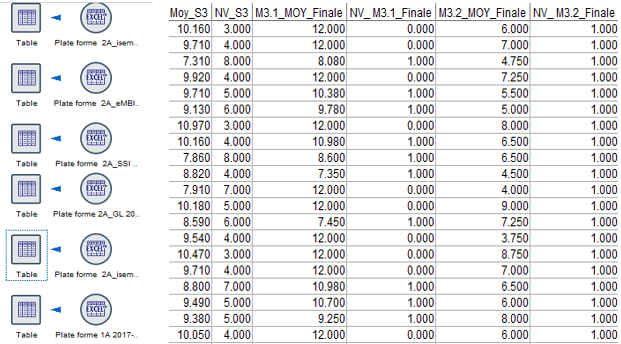
\includegraphics[scale=0.6]{fig5}}
                    \caption{Explorer les données à l’aide des tableaux}
                    \label{fig:5}
                \end{figure}
                \par Nous avons connecté un nœud tableau avec chaque nœud source pour visualiser les données.
            \subsubsection{Visualisation du pourcentage de réussite}
            Il sera utile de connaitre le pourcentage des gens qui ont réussi avec félicitation et le pourcentage des admis et aussi les autres catégories donc nous avons choisi d’explorer cette donnée.
            \begin{figure}[h!]
                \centering
                \fbox{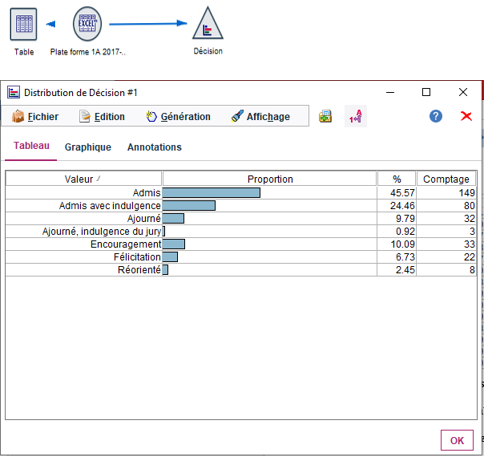
\includegraphics[scale=0.6]{fig6}}
                \caption{Pourcentage de réussite}
                \label{fig:6}
            \end{figure}
            D’après le résultat du nœud Distribution, la plupart des étudiants sont des admis. Ainsi nous avons constaté que nous avons seulement 22 étudiants qui réussirent avec félicitation , c’est-à-dire ils ont une note supérieure à 15.
            \subsubsection{Visualisation du pourcentage des filières}
            Il sera utile aussi de visualiser le pourcentage et le nombre des étudiants dans chaque filière. Pour savoir le nombre des groupes quand on aura. Pour cela nous avons ajouté un champ qui contient la filière de chaque étudiant en utilisant le nœud « calculer ». Mais avant nous allons extraire le champ « NOM », puisque dans le fichier des étudiants « GL » nous disposons seulement des noms des étudiants, avec le nœud « filter ».\par
            \begin{figure}[h!]
                \centering
                \fbox{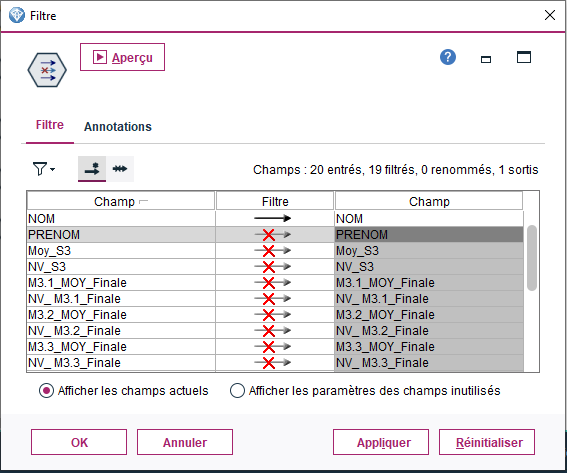
\includegraphics[scale=0.8]{fig7}}
                \caption{Extraire le champ des noms}
                \label{fig:7}
            \end{figure}
            \begin{figure}[h!]
                \centering
                \fbox{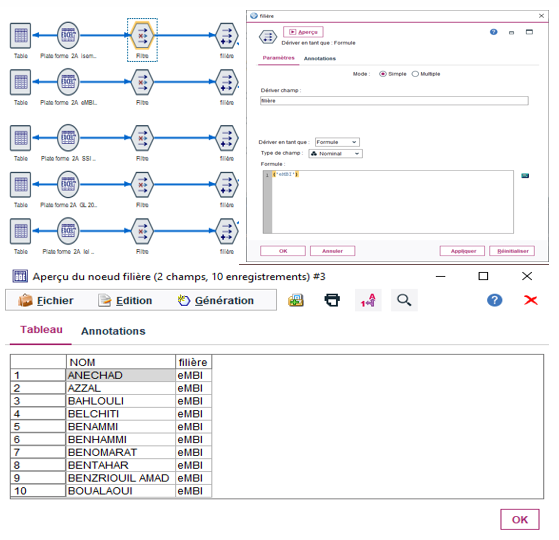
\includegraphics[scale=0.8]{fig8}}
                \caption{Ajouté la colonne de la filière}
                \label{fig:8}
            \end{figure}
            \newpage Puis on va faire une union entre les nœuds résultants et le nœud qui contient les notes de la première année avec le nœud « ajouter ».\par
            \begin{figure}[h!]
                \centering
                \fbox{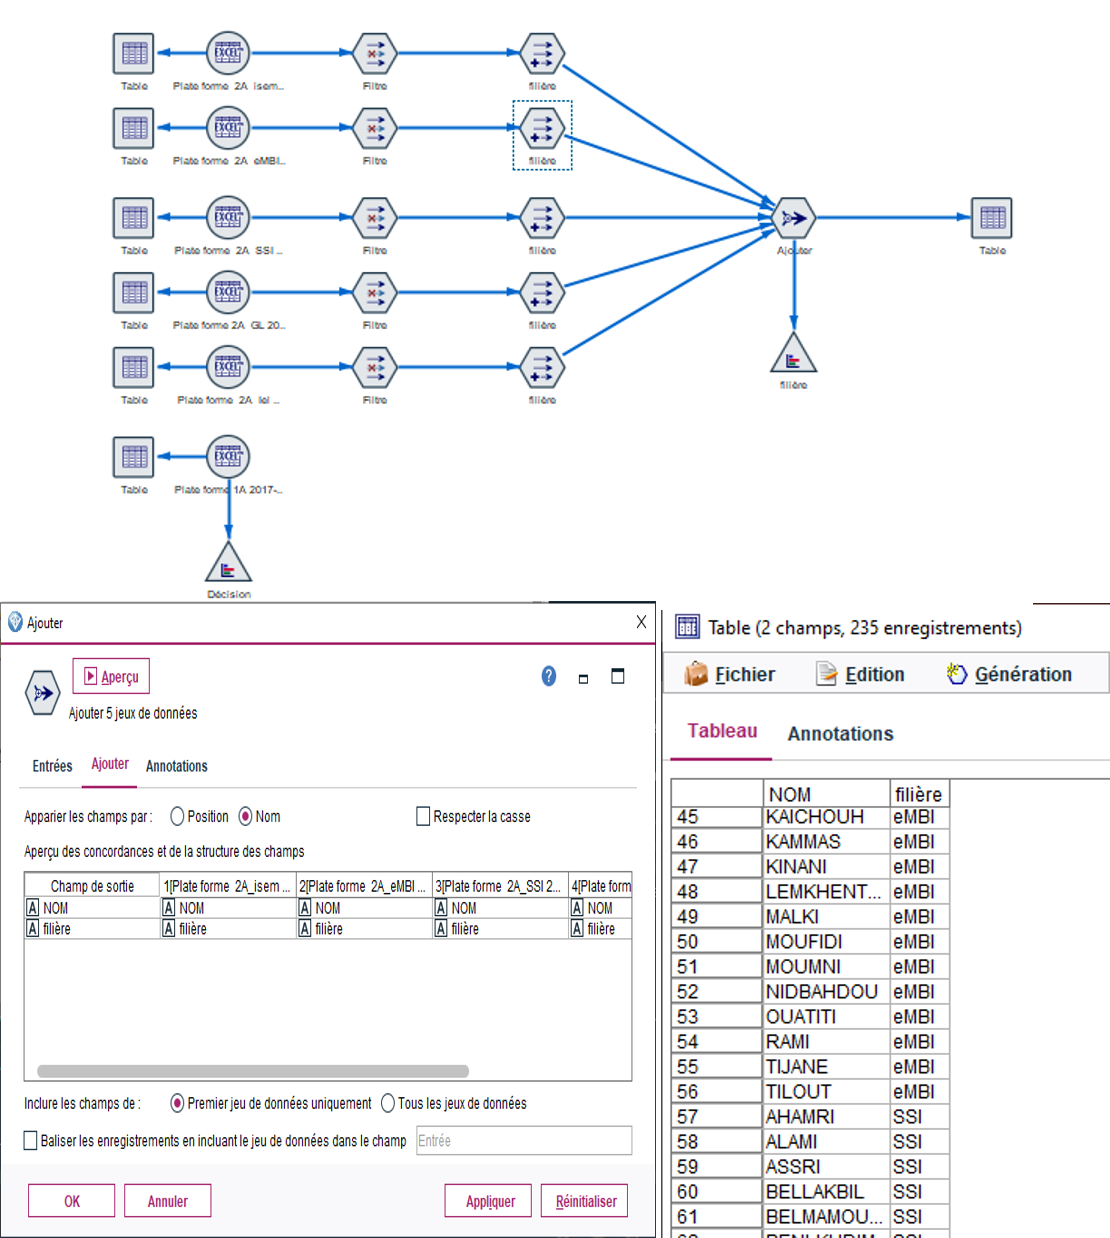
\includegraphics[scale=0.8]{fig9}}
                \caption{Union des nœuds}
                \label{fig:9}
            \end{figure}
            \begin{figure}[h!]
                \centering
                \fbox{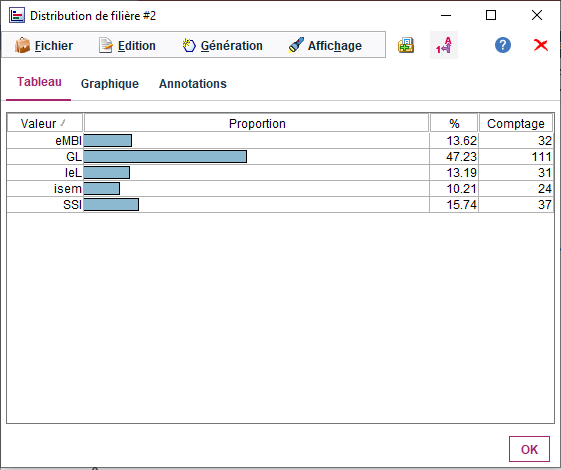
\includegraphics[scale=1]{fig10}}
                \caption{Pourcentage des filières}
                \label{fig:10}
            \end{figure}
            \newpage Nous avons remarqué que l’effectif des étudiants en « GL » est le plus grand. Par contre l’effectif en « Isem » est le plus petit. Ainsi on peut constater que les filières « eMBI », « Isem » contient un nombre pair des élèves donc on n’aura que des binômes. Par contre dans les autres filières, il y a un nombre impair des étudiants donc il y aura des monômes.
            \subsection{Vérification de la qualité des données}
            \par
            \begin{figure}[h!]
                \centering
                \fbox{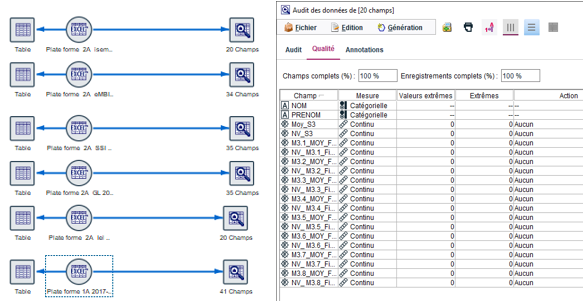
\includegraphics[scale=1]{fig11}}
                \caption{Qualité des données}
                \label{fig:11}
            \end{figure}
            Pour la qualité des données tous les fichiers ont des champs complets sauf le fichiers qui contient les notes de la filière SSI.
            \begin{figure}[h!]
                \centering
                \fbox{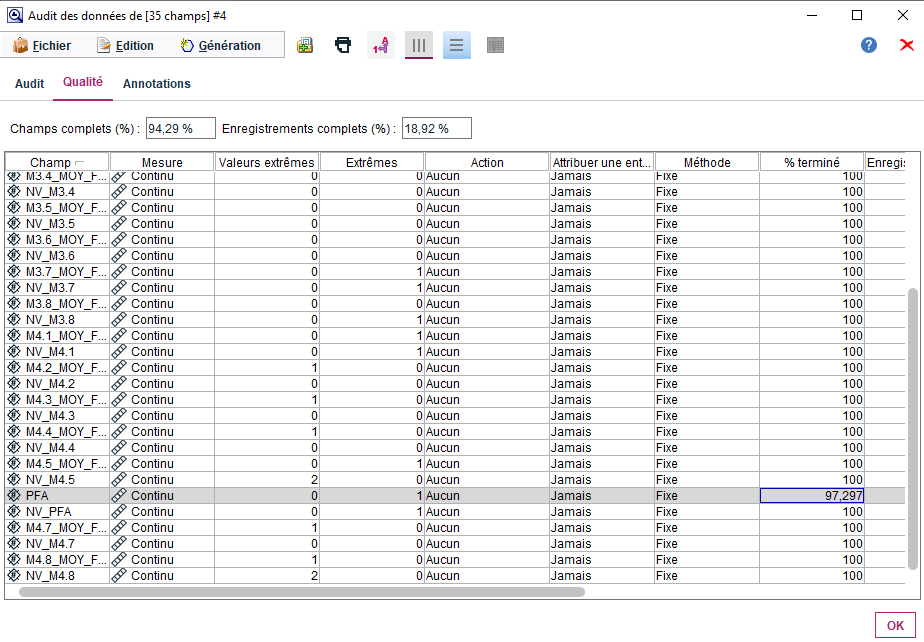
\includegraphics[scale=0.6]{fig12}}
                \caption{Qualité des données de nœud notes SSI}
                \label{fig:12}
            \end{figure}
            \newpage Il y’ a un manque des valeurs dans le champ status (30 valeurs manquantes) ainsi dans le champ PFA il y a une seule valeur manquante.
            \section{Préparation des données}
            La préparation des données est l’un des aspects les plus importante et les plus coûteux en temps du Data Mining. Dans cette section, on va voir la sélection des données, le nettoyage des donnés et l’intégration des données.
            \subsection{Sélection des données }
            Après avoir effectué la collecte initiale de données on doit maintenant choisir les données pertinentes pour nos objectifs de Data Mining.
            \par Les données que nous avons besoin sont : les noms et les prénoms des étudiants et leurs notes.
            \begin{figure}[h!]
                \centering
                \fbox{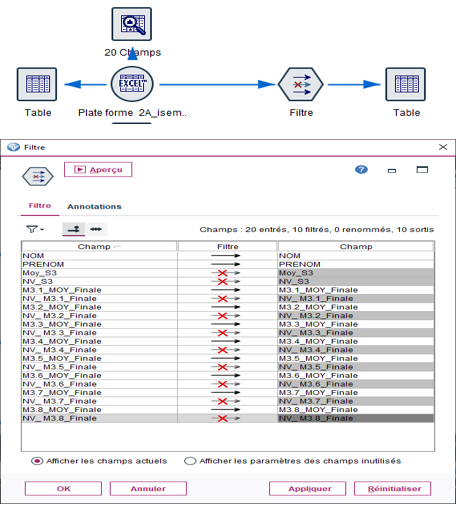
\includegraphics[scale=1]{fig13}}
                \caption{Sélection des données}
                \label{fig:13}
            \end{figure}
            \par Pour tous les fichiers, nous avons sélectionné les noms, les prénoms et les notes des étudiants dans les huit modules et nous avons éliminé les autres attributs en utilisant le nœud « Filter ». 
            \subsection{Nettoyage des données}
            \subsubsection{Données manquantes}
            Comme nous avons déjà montré dans le chapitre précédant il y a une seule valeur manquante. C’est la note du projet de la fin d’année (PFA) d’un étudiant dans la filière SSI. On va donc la remplacer avec la valeur moyenne.
            \begin{figure}[h!]
                \centering
                \fbox{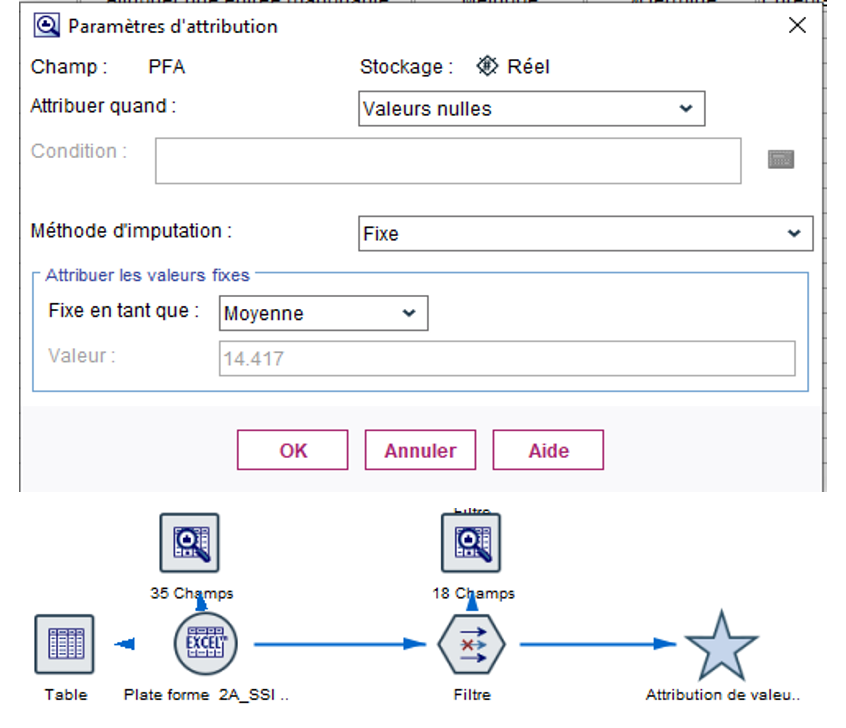
\includegraphics[scale=1]{fig14}}
                \caption{Insertion d'une valeur manquante}
                \label{fig:14}
            \end{figure}    
            \subsubsection{Erreurs dans les données}
            Nous avons vérifier manuellement les valeurs de telles manière que la valeur d’une note soit inclus entre 0 et 20. 
            \begin{figure}[h!]
                \centering
                \fbox{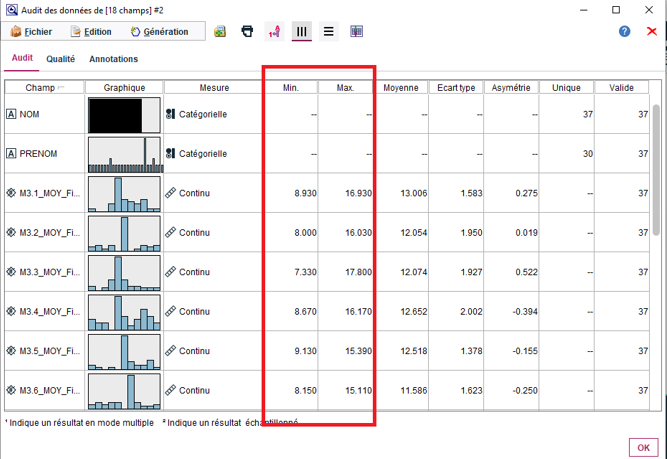
\includegraphics[scale=0.8]{fig15}}
                \caption{vérification des données}
                \label{fig:15}
            \end{figure}  
            \begin{figure}[h!]
                \centering
                \fbox{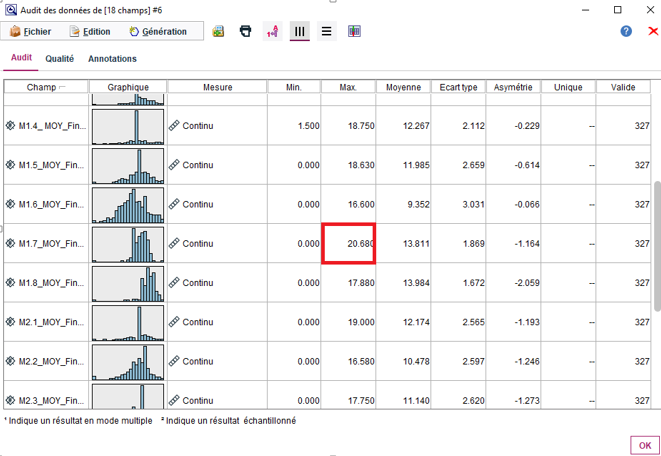
\includegraphics[scale=0.8]{fig16}}
                \caption{Détection d’une valeur erronée}
                \label{fig:16}
            \end{figure} 
            \newpage Nous avons trouvé une valeur anormale au niveau du module 1.7 dans les notes de la première année, la note est 20.68 ce qui est impossible.
            \begin{figure}[h!]
                \centering
                \fbox{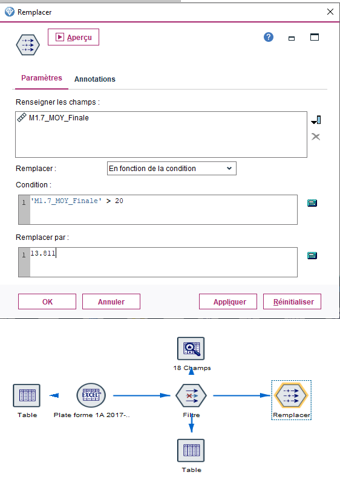
\includegraphics[scale=1]{fig17}}
                \caption{Remplacer la valeur erronée par la valeur moyenne}
                \label{fig:17}
            \end{figure} 
            \newpage On va remplacer cette valeur par la moyenne qui est 13.811.
            \subsection{Intégration des données}
            Il existe deux méthodes principales pour l’intégration des données : la fusion et l’ajout. Dans notre cas on va faire la fusion des données. Nous avons fusionné les ensembles de données de la première année avec les données de la deuxième année de chaque filière.
            \begin{figure}[h!]
                \centering
                \fbox{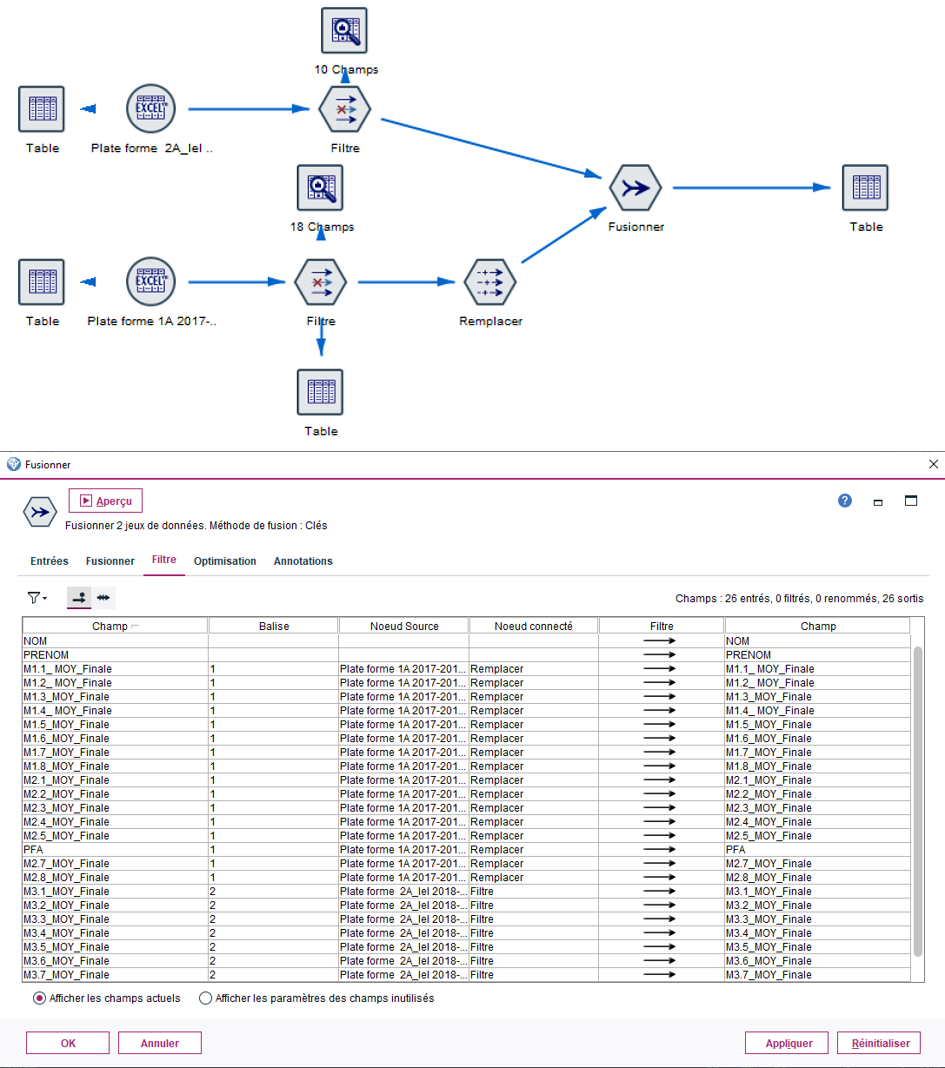
\includegraphics[scale=0.8]{fig18}}
                \caption{Fusionner les données de la première année et de la deuxième année de la filière Iel}
                \label{fig:18}
            \end{figure}    
            \newpage Par exemple dans la figure 18 on a la fusion des deux ensembles des données : les données de la première année et les données de la deuxième année des étudiants de la filière Iel.
            \newpage \section{Modélisation}
            La quatrième étape est la modélisation qui est au cœur de tout projet d'apprentissage automatique. Cette étape est responsable des résultats qui devraient satisfaire ou aider à atteindre les objectifs du projet.
            \par Bien que ce soit la partie glamour du projet, c'est aussi la plus courte dans le temps, car si tout ce qui précède est fait correctement, il y a peu à ajuster. Dans le cas où les résultats sont améliorables, la méthodologie est définie pour revenir à la préparation des données et améliorer les données disponibles.
            \par Dans ce chapitre, on va voir la sélection des techniques de modélisation, la géneration d’une conception de test et la construction du modèle.
            \subsection{Sélection des techniques de modélisation}
            Il y’ a plusieurs types de modélisation. Le choix du modèle le plus adéquat sera généralement basé sur les critères suivants :
            \begin{itemize}
                \item Les types de données disponibles pour l’exploration :
            \end{itemize}

                \newline Les champs inéressants sont numérique.
            \begin{itemize}
                \item Les objectifs de data mining :
            \end{itemize}
                \par Notre problème est un problème  de classification  non supervisé. Nous avons plusieurs méthodes de clustering : méthode hiérarchiques, méthodes de partitionnement, méthodes mixtes et analyse floue. 
                \newline Nous avons choisi de travailler avec l’algorithme de K-means : c’est une méthode de partitionnement. Il permet de regrouper en K clusters distincts les observations du data set.
                \par Nous avons choisi K-means pour ces raisons :
            \begin{itemize}
                \item Simple et robuste.
                \item On définit nous même le nombre de clusters.
                \item Efficace : O(n.t.k) avec n : le nombre des objets, t : nombre des itérations et k : le nombre des clusters.
            \end{itemize}
            \subsection{Géneration d’une conception de test}
            La dernière étape avant la création du modèle consiste à considérer la façon dont les résultats du modèle seront testés. Puisqu’on est dans le cas d’un modèle non supervisé le critère de « qualité d’ajustement » de notre modèle sera la taille des clusters. En effet nous voulons minimiser les groupes avec une seule personne. Ainsi il sera comme critère la facilité d’interpretation et le temps de traitement nécessaire.
            \subsection{Construire le modèle}
            Nous avons commencer par ajouter le noeaud « typer » pour les définir les données entrants du modèle.
            \begin{figure}[h!]
                \centering
                \fbox{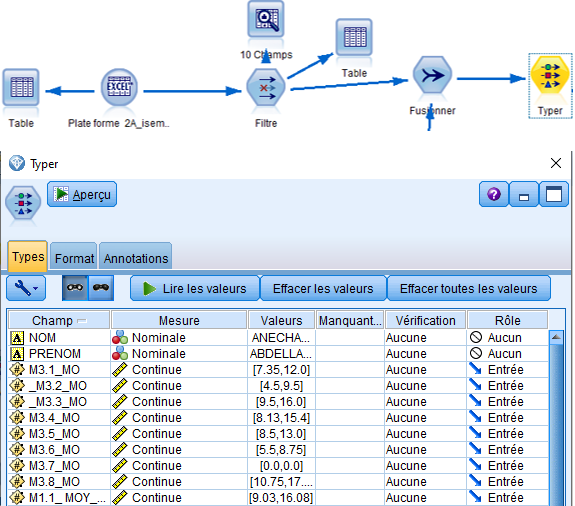
\includegraphics[scale=1]{fig19}}
                \caption{Définir les inputs du modèle}
                \label{fig:19}
            \end{figure}    
            \newpage Nous avons définit tous les champs comme des champs « entrée » sauf nom et prénom que nous avons défini leur rôle comme « aucun ».
            \begin{figure}[h!]
                \centering
                \fbox{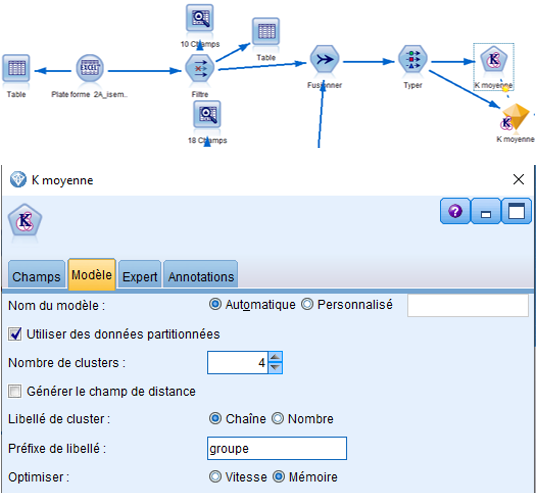
\includegraphics[scale=1]{fig20}}
                \caption{Géneration du modèle }
                \label{fig:20}
            \end{figure}  
            \newpage Nous avons fixé le nombre de clusters pour la filière isem sur 4.  Nous aurons donc 4 groupes des étudiants chaque groupe est constitué des étdudiants ayant des notes similaires.
            \begin{figure}[h!]
                \centering
                \fbox{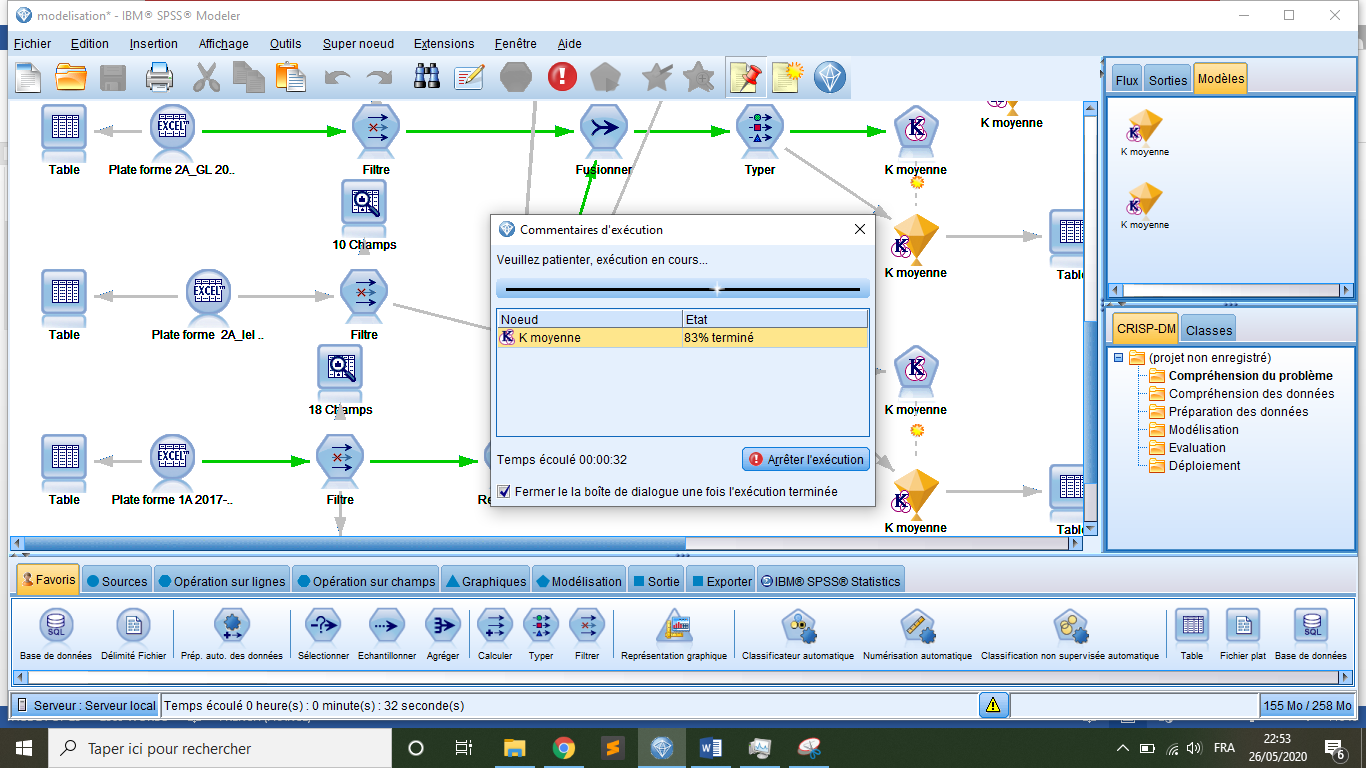
\includegraphics[scale=0.45]{fig21}}
                \caption{Temps d’exécution}
                \label{fig:21}
            \end{figure} 
            \newpage Pour le temps d’exécution, il est raisonnable par exemple dans le cas de la filière GL le temps d’exécution est 33 secondes
            \begin{figure}[h!]
                \centering
                \fbox{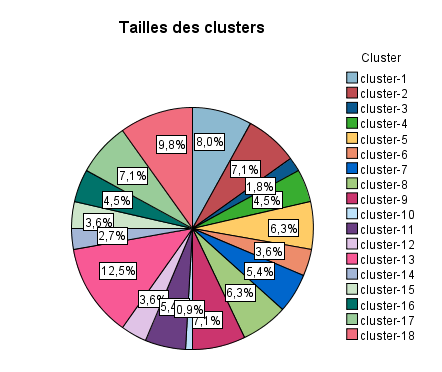
\includegraphics[scale=1]{fig22}}
                \caption{Taille des clusters}
                \label{fig:22}
            \end{figure} 
            \par Nous avons obtenu des clusters avec différents tailles. On a un seul cluster de taille 1. Donc nous avons atteint notre objectif.
            \begin{figure}[h!]
                \centering
                \fbox{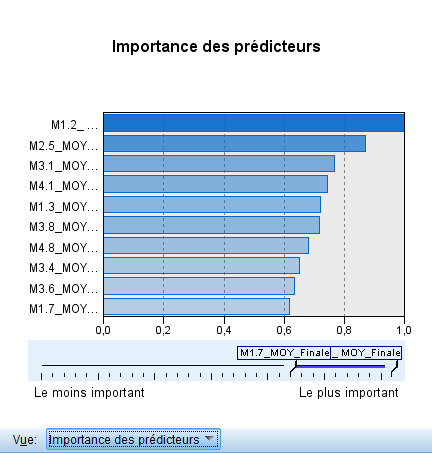
\includegraphics[scale=1.2]{fig23}}
                \caption{Importance des prédicteurs}
                \label{fig:23}
            \end{figure} 
            \par Dans le cas des étudiants de la filière Génie Logiciel (GL) le prédicteur le plus important est la note du module 1.2.
            \newpage \begin{figure}[h!]
                \fbox{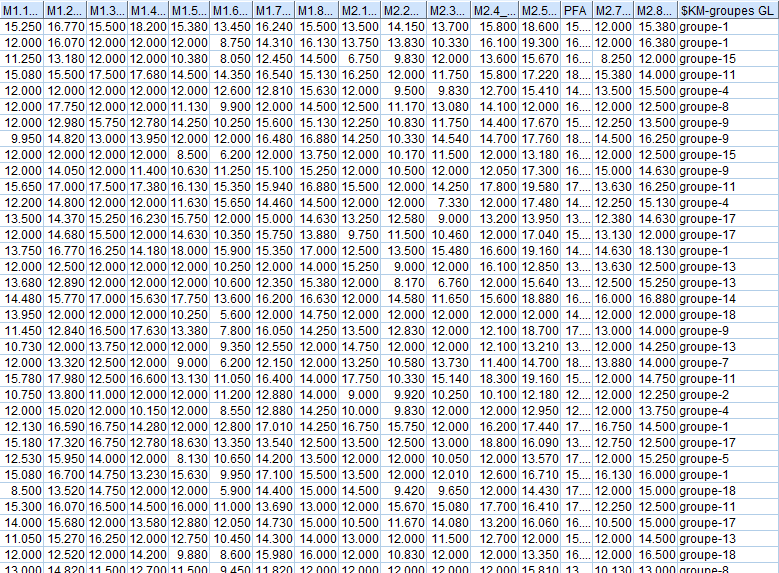
\includegraphics[scale=0.8]{fig24}}
                \caption{Résultat}
                \label{fig:24}
            \end{figure} 
            \newpage \section{Evaluation et déploiement}
            \subsection{Evaluation}
            \subsubsection{Qualité du modèle}
            Pour mésurer la qualité de notre modèle, nous prenons en considération la qualité des clusters. Dans notre cas, elle est correcte (Silhouette moyenne = 0.3).
            \begin{figure}[h!]
                \centering
                \fbox{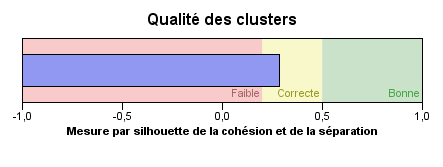
\includegraphics[scale=1.2]{fig25}}
                \caption{Qualité des clusters}
                \label{fig:25}
            \end{figure} 
            \subsubsection{Amélioration}
            Pour améliorer notre projet, il sera préférable d'obtenier des cluster de la même taille. Pour que les étudiant auront la même liberté de choisir leus groupes de travail.
            \subsection{Déploiement}
            Le déploiement est le processus consistant  à utiliser les nouvelles connaissances pour apporter des améliorations au sein de l'établissement. 
            \par Notre projet va aider les professeurs de l'ENSIAS à former des groupes homogènes des étudiants pour qu'ils puissent exploiter leurs compétences.
            
    \newpage
    \begin{center}
    \Large \textbf{Conclusion}
    \end{center}
    \begin{spacing}{2}
    \par A travers ce projet, nous avons pu en effet consolider les connaissances acquises et d’enrichir Notre expérience en matière de data mining. A travers le sujet choisi « Analyse des relevés de notes des étudiants de l’ENSIAS », on constate que le date mining peut être appliqué dans tous les domaines et s’avère utile pour tous les décideurs.
    \par Pour atteindre notre objectif nous avons mis en place la démarche CRISP-DM ( CRoss Industry Standard Process for Data Mining ). Il s’agit d’un modèle de processus de data mining qui décrit une approche communément utilisée par les experts en data mining pour résoudre les problèmes qui se posent à eux.
    \end{spacing}
    \newpage
    \begin{center}
    \Large \textbf{Références}
    \end{center}
    \begin{spacing}{2}
    \begin{enumerate}
        \item \large{\textbf{Cours Data Mining: Concepts et Techniques}}, de Madame Houda \newline Benbrahim
        \item \large{\textbf{Documentation de IBM SPSS Modeler}}, disponible sur : https://www.ibm.com/\newline support/knowledgecenter/SS3RA7\_sub/modeler\_kc\_subscription/ clementine/\newline knowledge\_center/product\_landing\_subscription.html
        \item \large{\textbf{Overleaf}} : Editeur de LaTex en ligne, disponible sur : https://fr.overleaf.com/
        \item \large{\textbf{Documentation de Overleaf}}, disponible sur :  overleaf.com/learn
    \end{enumerate}
    \end{spacing}
\end{document}
